% !Mode:: "TeX:UTF-8"
%!TEX program  = xelatex

\documentclass[bwprint,12pt,fontset=windows]{gmcmthesis}

\hypersetup{hidelinks}
\usepackage[framemethod=TikZ]{mdframed}

%\usepackage{fontspec}  % for Consolas & Courier New
%\lstset{basicstyle=\small\fontspec{Consolas}}
%\lstset{basicstyle=\small\fontspec{Courier New}}
%\setmonofont{Consolas}
%\setcounter{tocdepth}{3}   % 调整目录深度

\usepackage{subfig}
\usepackage{colortbl}
\definecolor{color1}{rgb}{0.78,0.88,0.99}
\definecolor{color2}{rgb}{0.36,0.62,0.84}
%\definecolor{color3}{rgb}{0.8235,0.8706,0.9373}
\definecolor{color3}{rgb}{0.88,0.92,0.96}
\definecolor{color4}{rgb}{0.96,0.97,0.98}%{0.9176,0.9373,0.9686}

% 算法
\usepackage[noend]{algpseudocode}
\usepackage{algorithmicx,algorithm}
\floatname{algorithm}{算法}
\renewcommand{\algorithmicrequire}{\textbf{输入:}}
\renewcommand{\algorithmicensure}{\textbf{输出:}}

%\numberwithin{equation}{section}
%\numberwithin{figure}{section}
%\numberwithin{table}{section}


\newcommand{\red}[1]{\textcolor{red}{#1}}
\newcommand{\blue}[1]{\textcolor{blue}{#1}}


%===================== 建模论文题目 ======================

\title{全国研究生数学建模竞赛论文标题}
\baominghao{\hspace{6em} 20220900001} %参赛队号
\schoolname{\hspace{5.8em} 西安邮电大学}%学校名称
\membera{\hspace{6em} 成员A 邓浩楠} %队员A
\memberb{\hspace{6em} 成员B 汪子轩} %队员B
\memberc{\hspace{6em} 成员C 李珂} %队员C

%=======================================================


\begin{document}

 %生成标题
 \maketitle

 %填写摘要
\begin{abstract}
本模板是为全国研究生数学建模竞赛编写的 \LaTeX{} 模板, 旨在让大家专注于
论文的内容写作, 而不用花费过多精力在格式的定制和调整上. 本手册是相应的参考, 其
中提供了一些环境和命令可以让模板的使用更为方便. 同时需要注意, 使用者需要有一
定的 \LaTeX{} 的使用经验, 至少要会使用 ctex 宏包的一些功能, 比如调节字距或修改字体
大小等等.


 \begin{mdframed} [%
	roundcorner=5pt,
	linecolor=gray!50,
	outerlinewidth=0.5pt,
	middlelinewidth=0.3pt, backgroundcolor=gray!2,
innertopmargin=\topskip, frametitle={2021年格式变化说明},
frametitlefont= \bfseries,frametitlerule=true,frametitlealignment =\raggedright\noindent,
frametitlerulewidth=.5pt, frametitlebackgroundcolor=gray!2,]
今年的格式变化如下:
\begin{enumerate}
\item 论文第一页为标识替换。
\end{enumerate}

\end{mdframed}

这是研究生报名官方网站,点击\href{https://cpipc.chinadegrees.cn}{\fbox{这里}}进入。


\keywords{折叠桌\quad  曲线拟合\quad   非线性优化模型\quad  受力分析}

\end{abstract}

\pagestyle{plain}

%目录 不推荐加
\maketoc

\clearpage

\section{问题重述}

\subsection{引言}   % 问题的背景

创意平板折叠桌注重于表达木制品的优雅和设计师所想要强调的自动化与功能性。为了增大有效使用面积。设计师以长方形木板的宽为直径截取了一个圆形作为桌面,又将木板剩余的面积切割成了若干个长短不一的木条,每根木条的长度为平板宽到圆上一点的距离,分别用两根钢筋贯穿两侧的木条,使用者只需提起木板的两侧,便可以在重力的作用下达到自动升起的效果,相互对称的木条宛如下垂的桌布,精密的制作工艺配以质朴的木材,让这件工艺品看起来就像是工业革命时期的机器。


\subsection{问题的提出}

%\subsubsection{问题的提出内容一}

\noindent 围绕创意平板折叠桌的动态变化过程、设计加工参数,本文依次提出如下问题:

\textbf{问题一:} 给定长方形平板尺寸 ($120 cm \times 50 cm \times 3 cm$),每根木条宽度(2.5 cm),连接桌腿木条的钢筋的位置,折叠后桌子的高度(53 cm)。要求建立模型描述此折叠桌的动态变化过程,并在此基础上给出此折叠桌的设计加工参数和桌脚边缘线的数学描述。


\textbf{问题二:} 折叠桌的设计应做到产品稳固性好、加工方便、用材最少。对于任意给定的折叠桌高度和圆形桌面直径的设计要求,讨论长方形平板材料和折叠桌的最优设计加工参数,例如,平板尺寸、钢筋位置、开槽长度等。对于桌高70 cm,桌面直径80 cm的情形,确定最优设计加工参数。


\textbf{问题三:} 给出软件设计的数学模型,可以根据客户任意设定的折叠桌高度、桌面边缘线的形状大小和桌脚边缘线的大致形状,给出所需平板材料的形状尺寸和切实可行的最优设计加工参数,使得生产的折叠桌尽可能接近客户所期望的形状,并根据所建立的模型给出几个设计的创意平板折叠桌。要求给出相应的设计加工参数,画出至少8张动态变化过程的示意图。



\clearpage
\section{模型的假设}

\begin{enumerate}
\item 忽略实际加工误差对设计的影响;
\item 木条与圆桌面之间的交接处缝隙较小,可忽略;
\item 钢筋强度足够大,不弯曲;
\item 假设地面平整。
\end{enumerate}


\section{符号说明}

\begin{table}[htp!]
\centering
\renewcommand\arraystretch{1.2} %定义表格高度
\newcolumntype{L}{>{\quad}X}
\newcolumntype{P}[1]{>{\centering\arraybackslash}p{#1}}
\newcolumntype{C}{>{\centering \arraybackslash}X}
\newcolumntype{R}{>{\raggedright \arraybackslash}X}
\begin{tabularx}{0.9\textwidth}{|P{1cm}|L|}
  \hline %\toprule
  符号    &   \quad 意义 \\
  \hline %\midrule
  %\rowcolor[gray]{0.90}
  $ a $  &  符号1的意义    \\
  \hline
  $ b $  &  符号2的意义    \\
  \hline
  $ c $  &  符号3的意义符号3的意义    \\
  \hline
  $ d $  &  符号4的意义    \\
  \hline
  $ e $  &  符号5的意义     \\
  \hline
  $ f $  &  符号6的意义符号6的意义    \\
  \hline
  $ g $  &  符号7的意义     \\
  \hline
  $ h $  &  符号8的意义     \\
  \hline
  $ i $  &  符号9的意义符号9的意义     \\
  \hline

  $ k $  &  符号10的意义     \\
  \hline
  $ l $  &  符号11的意义    \\
  \hline
  $ m $  &  符号12的意义    \\
  \hline
  $ n $  &  符号13的意义    \\
  \hline
  $ p $  &  符号14的意义    \\
  \hline
  $ q $  &  符号15的意义    \\
  \hline %\bottomrule
\end{tabularx}
\end{table}


%\begin{tabularx}{\textwidth-18pt}{XXX}
%\hline
%Input & Output& Action return \\
%\hline
%DNF &  simulation & jsp\\
%\hline
%\end{tabularx}


\section{模型的建立}

\subsection{问题一分析}
题目要求建立模型描述折叠桌的动态变化图,由于在折叠时用力大小的不同,我们不能描述在某一时刻折叠桌的具体形态,但我们可以用每根木条的角度变化来描述折叠桌的动态变化。首先,我们知道折叠桌前后左右对称,我们可以运用几何知识求出四分之一木条的角度变化。最后,根据初始时刻和最终形态两种状态求出桌腿木条开槽的长度


\subsection{算法示例}

数学建模求解算法示例:

\begin{center}
\begin{minipage}{0.8\textwidth}
\begin{algorithm}[H]%[!htp]
\caption{算法的名字} %算法的名字
{\bf 输入:} %算法的输入, \hspace*{0.02in}用来控制位置,同时利用 \\ 进行换行
input parameters A, B, C\\
{\bf 输出:} %算法的结果输出
output result
\begin{algorithmic}[1]
\State some description 算法介绍 % \State 后写一般语句
\For{condition} % For 语句,需要和EndFor对应
  \State ...
  \If{condition} % If 语句,需要和EndIf对应
    \State ...
  \Else
    \State ...
  \EndIf
\EndFor
\While{condition} % While语句,需要和EndWhile对应
  \State ...
\EndWhile
\State \Return result
\end{algorithmic}
\end{algorithm}
\end{minipage}
\end{center}


\section{表格和图形}

\subsection{表格}

%\begin{table}[!htbp]
%    \caption{标准三线表格}\label{tab:001} \centering
%    \begin{tabular}{ccccc}
%        \toprule%[1.5pt]
%        $D$(in) & $P_u$(lbs) & $u_u$(in) & $\beta$ & $G_f$(psi.in)\\
%        \midrule%[1pt]
%        5 & 269.8 & 0.000674 & 1.79 & 0.04089\\
%        10 & 421.0 & 0.001035 & 3.59 & 0.04089\\
%        20 & 640.2 & 0.001565 & 7.18 & 0.04089\\
%        \bottomrule%[1.5pt]
%    \end{tabular}
%\end{table}

三线表

\begin{table}[!htp]
\newcolumntype{L}{X}
\newcolumntype{C}{>{\centering \arraybackslash}X}
\newcolumntype{R}{>{\raggedright \arraybackslash}X}
\centering
\caption{某校学生升高体重样本}
\label{tab2:heightweight}
\begin{tabularx}{0.9\textwidth}{CCCC}
   \toprule
	序号&年龄&身高&体重\\
	\midrule
	1&14&156&42\\
	2&16&158&45\\
	3&14&162&48\\
	4&15&163&50\\
    \midrule
    %\cmidrule{2-4}
	平均&15&159.75&46.25\\
	\bottomrule
\end{tabularx}
\end{table}

某行业产量与生产费用的数据
\begin{table}[htp!]
\centering
\caption{某行业产量与生产费用的数据}%\label{}
\newcolumntype{Y}{>{\centering\arraybackslash}X}
\newcolumntype{Z}{!{\vline}@{\color{white}\vrule width \doublerulesep}!{\vrule}}%自定义列格式(双线)
\begin{tabularx}{0.9\textwidth}{c|c|YZc|c|Y}\Xhline{0.9pt}
	企业编号&	产量(台)&生产费用(万元)&企业编号&产量(台)&生产费用(万元)\\\Xcline{1-3}{0.6pt}\Xcline{4-6}{0.6pt}
	1&	40&	130&7&	84&	165\\
	2&	42&	150&8&	100&	170\\
	3&	50&	155&9&	116&	167\\
	4&	55&	140&10&	125&	180\\
	5&	65&	150&11&	130&	175\\
	6&	78&	154&12&	140&	185\\\Xhline{0.72pt}
\end{tabularx}
\end{table}

研究生数学建模2019年F题结果示例
\begin{table}[htp!]
\centering
\caption{问题1结果1 (左) 与 问题2结果 (右)}
\begin{minipage}[h]{0.48\linewidth}
\renewcommand\arraystretch{1.2} %定义表格高度
\newcolumntype{Y}{>{\centering\arraybackslash}X}
\begin{tabularx}{0.9\textwidth}{|Y|Y|Y|}
  \hline
  数据集1  &  数据集1 & 数据集2  \\
 \hline
  A问题1   & A问题1 &  A问题1     \\
  \hline
  503   &  503     & 163     \\
  294   &  200     & 114      \\
  91    &  80      & 8     \\
  607   &  237     & 309      \\
  540   &  170     & 305    \\
  250   &  278     & 123    \\
  340   &  369     & 45      \\
  277   &  214     & 160    \\
  B     &  397     & 92    \\
        &  B       & 93    \\
        &          & 61        \\
        &          & 292       \\
        &          & B         \\
104861  & 103518   & 109342 \\
\hline
\end{tabularx}
\end{minipage}
\begin{minipage}[h]{0.48\linewidth}
\renewcommand\arraystretch{1.2} %定义表格高度
\newcolumntype{Y}{>{\centering\arraybackslash}X}
\begin{tabularx}{0.9\textwidth}{|Y|Y|Y|}
  \hline
  数据集1  &  数据集1 & 数据集2  \\
  \hline
  A问题2  &  A问题2  & A问题2    \\
  \hline
   503    & 503     & 163  \\
  294    & 200     & 114   \\
   91     & 80     & 8   \\
   607    & 237     & 309   \\
   540    & 170    & 305  \\
   250    & 278    & 123  \\
   340    & 369     & 45   \\
   277    & 214    & 160  \\
  B      & 397   & 92 \\
        &  B     &  93      \\
         &         &  61      \\
        &         &   292     \\
        &         &   B     \\
 104917  &  103563  &109427 \\
\hline
\end{tabularx}
\end{minipage}
\end{table}


\begin{table}[htp!]
%\small
\centering
\renewcommand\arraystretch{1.2} %定义表格高度
\newcolumntype{Y}{>{\centering\arraybackslash}X}
\caption{问题3结果}
\begin{tabularx}{0.9\textwidth}{|Y|Y|Y|Y|Y|Y|}
  \hline %定义表格宽度
  数据集1  &  数据集1  &  \multicolumn{2}{c|}{数据集2 (无问题点)}  & \multicolumn{2}{c|}{数据集2 (有问题点)} \\
  \hline
  A问题3   & A问题3   &  \multicolumn{2}{c|}{A问题3}    &  \multicolumn{2}{c|}{A问题3}      \\
  \hline
  503      & 503     & 169      & 73      & 169     & 73   \\
  \hline
  69       & 69      & 322      & 249     & 322     & 249   \\
  \hline
  506      & 506      & 270     & 274     & 270     & 274   \\
  \hline
  371      & 371      & 89      & 12      & 89      & 12   \\
  \hline
  183      & 183      & 236     & 216     & 236     & 216  \\
  \hline
  194      & 194      & 132     & 16      & 132     & 16   \\
  \hline
  450      & 450      & 53      & 282     & 53      & 282   \\
  \hline
  286      & 113      & 112     & 84      & 112     & 141  \\
  \hline
  485      & 485      &  268    & 287     & 268     & 291 \\
  \hline
 \red{B (9D)}~~     & 248      & 250     & 99      & 250     &161 \\
 \hline
   & \red{B (10D)}   & 243     & \red{B (21D)}   & 243    & \red{B (21D)} \\
   \hline
    &          &         &         &         &       \\
    \hline
  104861m  & 103518m  &         & 168924m  &         &161650m \\
\hline
\end{tabularx}
\end{table}


\clearpage
\subsection{图形}

图形并列
\begin{figure}[htp!]
\begin{minipage}[t]{0.48\linewidth}
\centering
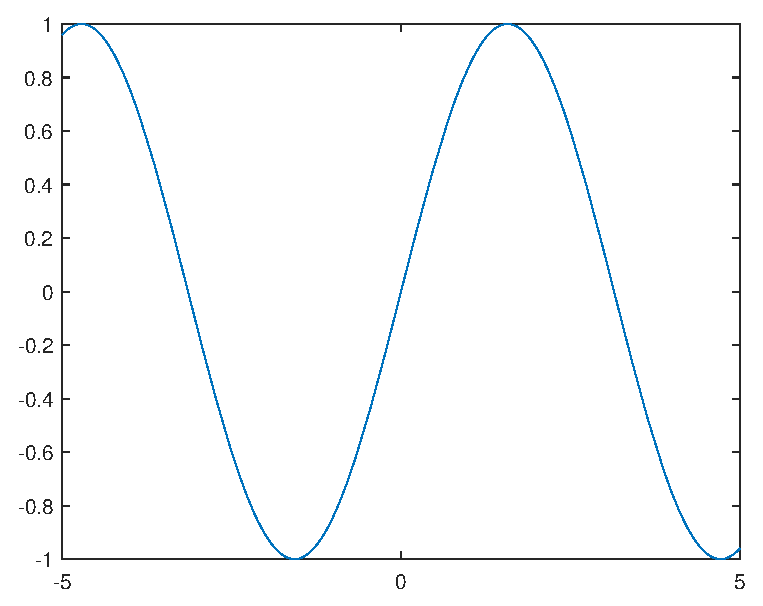
\includegraphics[width=0.9\textwidth]{image1}
\caption{fig1}
\label{fig:side:a}
\end{minipage}%
\begin{minipage}[t]{0.48\linewidth}
\centering
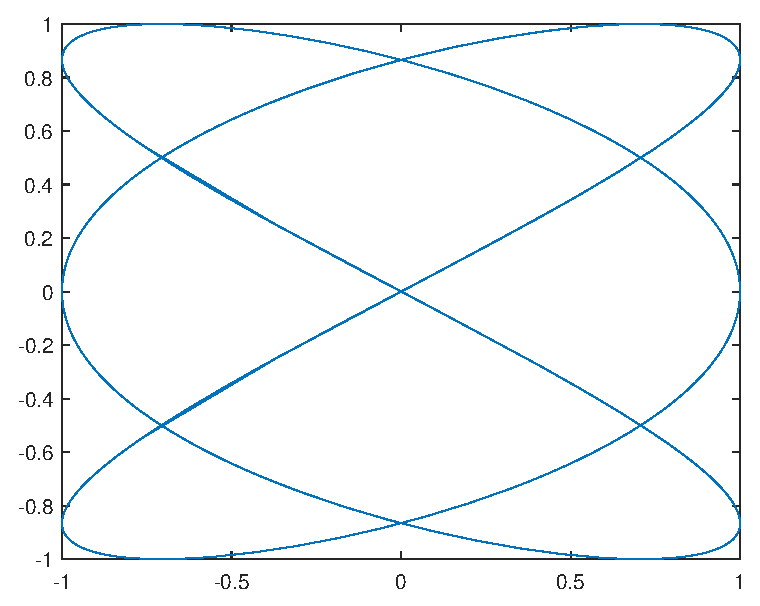
\includegraphics[width=0.9\textwidth]{image2}  % 2.2in
\caption{fig2}
\label{fig:side:b}
\end{minipage}
\end{figure}

这是一个算法流程图
\begin{figure}[htp!]
\centering
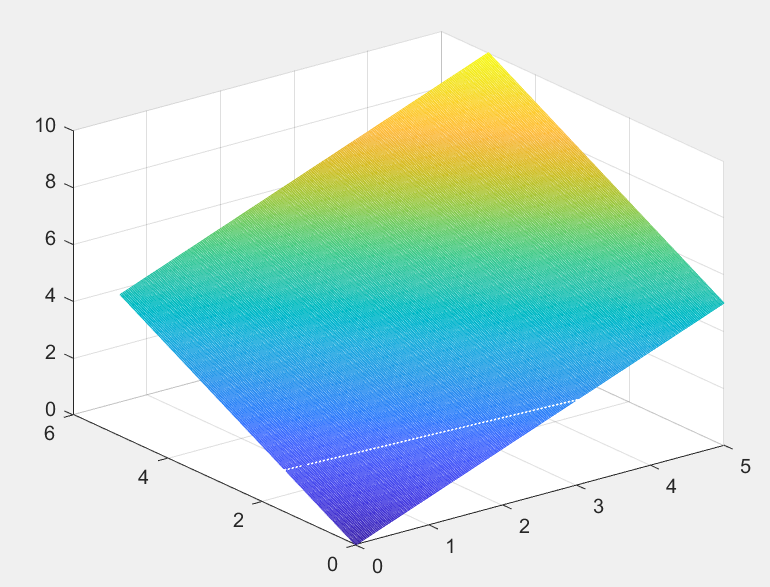
\includegraphics[width=.7\textwidth]{1.png}
\caption{算法流程图}
\end{figure}

\clearpage
\begin{figure}[!htp]
	\centering
	\subfloat[Arabic numerals]{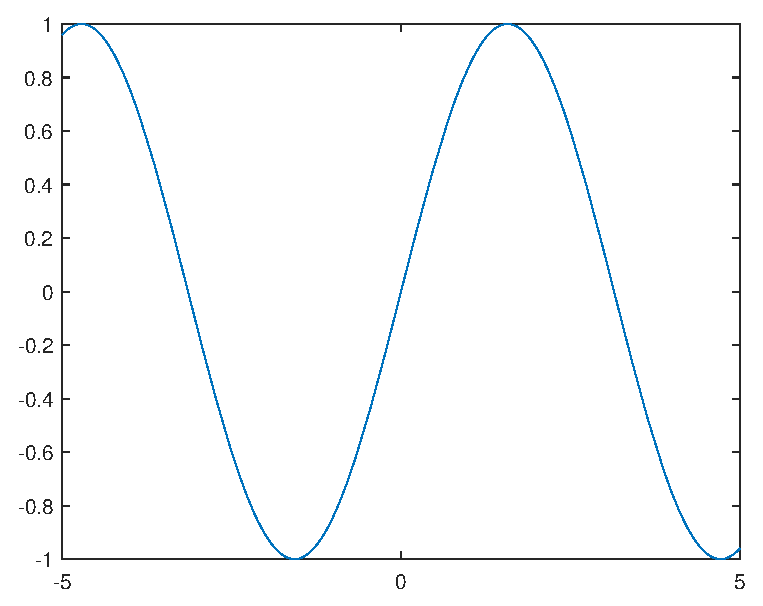
\includegraphics[width=0.4\textwidth]{image1}}\qquad
	\subfloat[Arabic numerals]{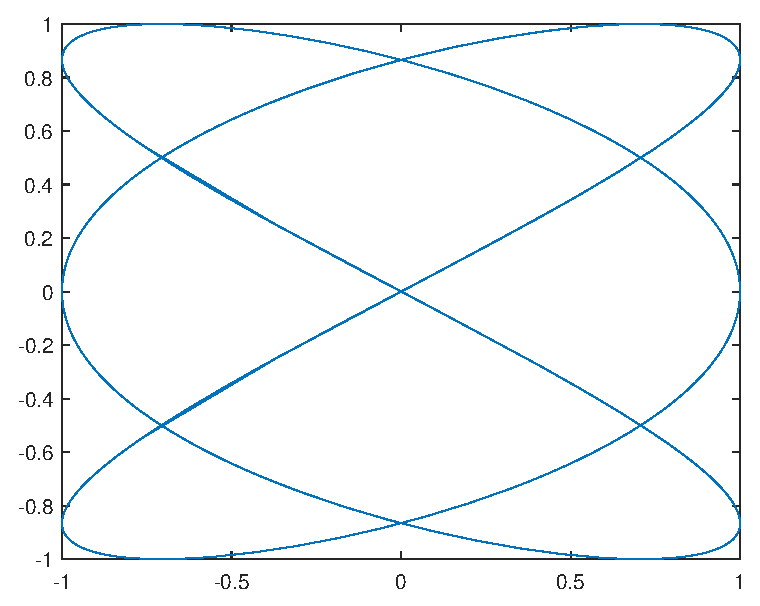
\includegraphics[width=0.4\textwidth]{image2}} \\
	\subfloat[Arabic numerals]{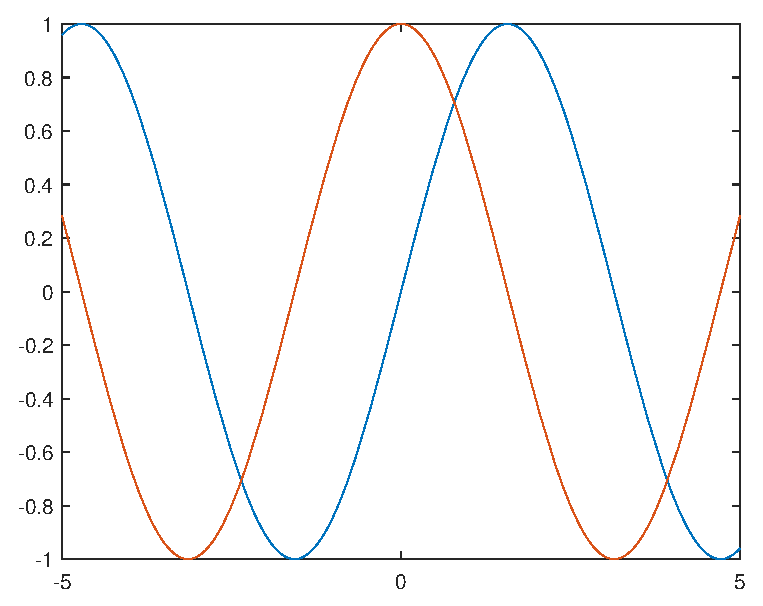
\includegraphics[width=0.4\textwidth]{image3}}\qquad
	\subfloat[Arabic numerals]{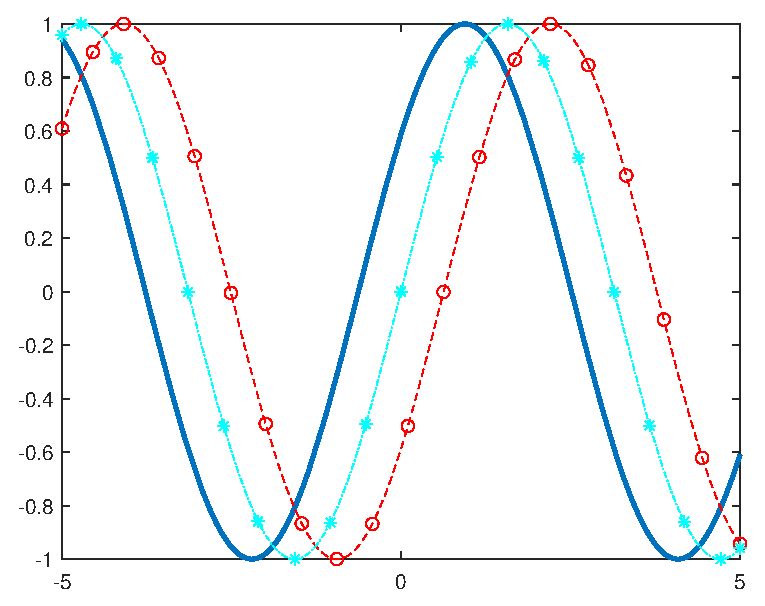
\includegraphics[width=0.4\textwidth]{image4}}
	\caption{多图示例}
\end{figure}


\subsection{问题三分析}


题目要求制作软件的意思就是客户给定折叠桌高度、桌面边缘线的形状大小和桌脚边缘线的大致形状,将这些信息输入程序就得到客户想要的桌子。我们在求解最优设计加工参数时,自行给定桌面边缘线形状(椭圆、相交圆等),桌脚边缘线形状,折叠桌高度,应用第二问的非线性规划模型,用MATLAB软件绘制折叠桌截面图,得到自己设计的创意平板折叠桌。


\section{模型评价}

这里是模型评价



%参考文献   手工录入
%\begin{thebibliography}{9}%宽度9
% \bibitem{bib:one} ....
% \bibitem{bib:two} ....
%\end{thebibliography}

%采用bibtex方案
\cite{mittelbach_latex_2004,wright_latex3_2009,beeton_unicode_2008,vieth_experiences_2009}

\bibliographystyle{gmcm}
\bibliography{reference}


\clearpage
%附录
\begin{appendices}
%\setcounter{page}{1} %如果需要可以自行重置页码。
\section{MATLAB 源程序}
\renewcommand{\thesubsection}{A\thinskip.\thinskip\arabic{subsection}}
\subsection{第1问程序}
\vspace{-2ex}

\begin{Matlab}{code.m}
clear all
kk=2;
[mdd,ndd]=size(dd);
while ~isempty(V)
    [tmpd,j]=min(W(i,V));
    tmpj=V(j);
    for k=2:ndd
        [tmp1,jj]=min(dd(1,k)+W(dd(2,k),V));
        tmp2=V(jj);
        tt(k-1,:)=[tmp1,tmp2,jj];
    end
    tmp=[tmpd,tmpj,j;tt];
    [tmp3,tmp4]=min(tmp(:,1));
    if tmp3==tmpd,
        ss(1:2,kk)=[i;tmp(tmp4,2)];
    else
        tmp5=find(ss(:,tmp4)~=0);
        tmp6=length(tmp5);
        if dd(2,tmp4)==ss(tmp6,tmp4)
            ss(1:tmp6+1,kk)=[ss(tmp5,tmp4);tmp(tmp4,2)];
        else, ss(1:3,kk)=[i;dd(2,tmp4);tmp(tmp4,2)];
        end
    end
    dd=[dd,[tmp3;tmp(tmp4,2)]];
    V(tmp(tmp4,3))=[];
    [mdd,ndd]=size(dd);kk=kk+1;
end;
S=ss; D=dd(1,:);
\end{Matlab}
\vspace{2ex}

\clearpage
\section{Python 源程序}
\renewcommand{\thesubsection}{B\thinskip.\thinskip\arabic{subsection}}
\subsection{第2问程序}
\vspace{-2ex}
\begin{Python}{mip1.py}
# This example formulates and solves the following simple MIP model:
#  maximize
#        x +   y + 2 z
#  subject to
#        x + 2 y + 3 z <= 4
#        x +   y       >= 1
#        x, y, z binary

# import gurobipy as gp
from gurobipy import * #GRB
try:
    # Create a new model
    m = Model("mip1")
    # Create variables
    x = m.addVar(vtype=GRB.BINARY, name="x")
    y = m.addVar(vtype=GRB.BINARY, name="y")
    z = m.addVar(vtype=GRB.BINARY, name="z")
    # Set objective
    m.setObjective(x + y + 2 * z, GRB.MAXIMIZE)
    # Add constraint: x + 2 y + 3 z <= 4
    m.addConstr(x + 2 * y + 3 * z <= 4, "c0")
    # Add constraint: x + y >= 1
    m.addConstr(x + y >= 1, "c1")
    # Optimize model
    m.optimize()
    for v in m.getVars():
        print('%s %g' % (v.varName, v.x))
    print('Obj: %g' % m.objVal)

except GurobiError as e:
    print('Error code ' + str(e.errno) + ': ' + str(e))

except AttributeError:
    print('Encountered an attribute error')
\end{Python}

\end{appendices}



\end{document}
